% Fundamentação teórica

Linguagem de Programa\ca o \eh\ a nota\ca o utilizada para descrever computa\co es, comumente chamadas de programa de computador, para uma m\ah quina autom\ah tica e para pessoas. Antes que um programa possa ser utilizado, faz-se necess\ah ria a tradu\ca o do programa de computador para uma forma que uma m\ah quina autom\ah tica possa compreender.

O software respons\ah vel pela tradução do programa de computador \eh\ chamado compilador. Similar ao compilador, existe também o interpretador, capaz de utilizar o programa de computador em sua nota\ca o original (programa \emph{fonte}) e executar suas instru\co es diretamente.

%Contudo, h\ah\ de se notar que existe uma clara diferen\c{c}a nos objetivos dessas m\ah quinas virtuais. Portanto, \eh\ mais correto chamar as \"m\ah quinas virtuais\" de ambientes de execu\ca o de plataforma virtual.

\begin{figure}[!htbp]
  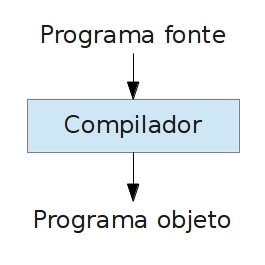
\includegraphics[width=0.15\textwidth]{figuras/compilador}
  \caption{O funcionamento de um compilador}
  \label{fig:compilador}
\end{figure}

Na figura \ref{fig:compilador} h\ah\ um esquema do funcionamento geral de um compilador, que recebe uma entrada na linguagem \emph{fonte}, e traduz para um programa equivalente na linguagem \emph{objeto}.

% \begin{figure}[here]
%   
\includegraphics[width=0.6\textwidth]{figuras/execucao}
%   \caption{Ambiente de execu\ca o de um programa de computador}
%   \label{fig:execucao}
% \end{figure}

Na figura \ref{fig:execucao} \eh\ poss\ih vel ver o funcionamento de um programa em funcionamento.

% \begin{figure}[here]
%   
\includegraphics[width=0.6\textwidth]{figuras/interpretador}
%   \caption{Um interpretador}
%   \label{fig:interpretador}
% \end{figure}

Na figura \ref{fig:interpretador}, o modelo de um interpretador.

% \begin{figure}[here]
%   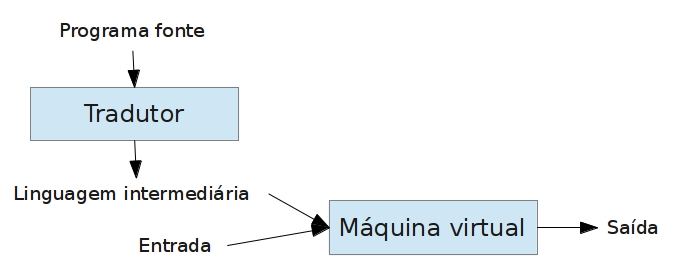
\includegraphics[width=0.6\textwidth]{figuras/hibrido}
%   \caption{Software h\ih brido}
%   \label{fig:hibrido}
% \end{figure}

J\ah\ na figura \ref{fig:hibrido}, o esquema de uma abordagem h\ih brida.

M\ah quina Virtual, conforme convencionou-se, \eh\ o software capaz de simular o comportamento de uma m\ah quina autom\ah tica, com a capacidade de ampliar a capacidade real da m\ah quina hospedeira.
As m\ah quinas virtuais podem servir a dois objetivos principais:
\begin{description}
\item[Amplia\ca o de hardware] Amplia a capacidade computacional de uma m\ah quina f\ih sica, disponibilizando ao software hospedado, mais mem\oh ria e/ou processadores do que realmente existem.
\item[Homogeneiza\ca o de ambiente de execu\ca o] Padroniza o ambiente de execuc\ca o do programa, muitas vezes permitindo que um mesmo programa possa ser reutilizado em v\ah rias plataformas sem nenhuma ou com poucas altera\co es.
\end{description}

Um exemplo de software compilador, \eh\ o {GCC\footnote{GNU Compiler Collection}}, que \eh\ capaz de interpretar as linguagens de programa\ca o C, C++, Fortran, Objective-C, entre outras.
Um exemplo de interpretador \eh\ o Python, que d\ah\ nome tamb\eh m \`a linguagem de programa\ca o.
Exemplos de abordagem h\ih brida, utilizando um compilador e um interpretador, s\ao as plataformas Java e .NET, que possuem um compilador, respons\ah vel por traduzir o programa fonte em uma representa\ca o intermedi\ah ria, comumente chamada de \emph{bytecode}; e um interpretador, comumente chamado de m\ah quina virtual, nomeadas {JVM\footnote{Java Virtual Machine}} e {mscorelib\footnote{mscorelib, respons\ah vel por interpretar os bytecodes da plataforma .NET}}, respectivamente.
